\documentclass{beamer}
\usetheme{Madrid} % Clean theme
\usepackage{listings}
\usepackage{xcolor}
\usepackage{graphicx}

\usepackage{gvv}

% Code listing style
\lstset{
  basicstyle=\ttfamily\footnotesize,
  keywordstyle=\color{blue},
  stringstyle=\color{orange},
  commentstyle=\color{green!60!black},
  breaklines=true,
  frame=single,
  showstringspaces=false
}

\title{MatGeo Assignment - Problem 4.7.8}
\author{EE25BTECH11024}
\institute{IIT Hyderabad}

\begin{document}

% Title slide
\begin{frame}
  \titlepage
\end{frame}

% Problem statement
\begin{frame}{Problem Statement}
Find the shortest distance between the lines
\begin{align}
\vec{l_1}: \vec{r}_1 = \hat{\vec{i}} + \hat{\vec{j}} + \lambda (2\hat{\vec{i}} - \hat{\vec{j}} + \hat{\vec{k}}), \quad
\vec{l_2}: \vec{r}_2 = 2\hat{\vec{i}} + \hat{\vec{j}} - \hat{\vec{k}} + \mu (3\hat{\vec{i}} - 5\hat{\vec{j}} + 2\hat{\vec{k}})
\label{eq:given}
\end{align}
\end{frame}


\begin{frame}{Formula Used}
    Least squares solution.
\begin{align}
\vec{M}^\top\vec{M}\myvec{\kappa_1 \\ -\kappa_2} = \vec{M}^\top(\vec{B} - \vec{A})
\label{eq:formula}
\end{align}
    
\end{frame}

\begin{frame}{Solution: }
\noindent
In this case, the given lines are
\begin{align}
    \vec{x} &= \myvec{1 \\ 1 \\ 0} + \kappa_1 \myvec{2 \\ -1 \\ 1} \label{eq:1} \\
    \vec{x} &= \myvec{2 \\ 1 \\ -1} + \kappa_2 \myvec{3 \\ -5 \\ 2} \label{eq:2}
\end{align}
with
\begin{align}
    \vec{A} = \myvec{1 \\ 1 \\ 0}, \quad \vec{B} = \myvec{2 \\ 1 \\ -1}, \quad \vec{M} = \myvec{2 & 3 \\ -1 & -5 \\ 1 & 2}
\end{align}
Then,
\begin{align}
    \vec{B} - \vec{A} = \myvec{1 \\ 0 \\ -1}
\end{align} 

\end{frame}

\begin{frame}{Solution: }
\noindent
Calculating the rank of  matrix \myvec{\vec{M} & \vec{B} - \vec{A}},

\begin{align*}
    \myvec{2 & 3 & 1 \\ -1 & -5 & 0 \\ 1 & 2 & -1} 
    &\xrightarrow{R_1 \leftrightarrow R_3} \myvec{1 & 2 & -1 \\ -1 & -5 & 0 \\ 2 & 3 & 1} 
    \xrightarrow{\substack{R_2 \to R_2 + R_1 \\ R_3 \to R_3 - 2R_1}} \myvec{1 & 2 & -1 \\ 0 & -3 & -1 \\ 0 & -1 & 3} \\
    &\xrightarrow{R_2 \leftrightarrow R_3} \myvec{1 & 2 & -1 \\ 0 & -1 & 3 \\ 0 & -3 & -1}
    \xrightarrow{R_2 \to -R_2} \myvec{1 & 2 & -1 \\ 0 & 1 & -3 \\ 0 & -3 & -1} 
    \xrightarrow{\substack{R_1 \to R_1 - 2R_2 \\ R_3 \to R_3 + 3R_2}} \myvec{1 & 0 & 5 \\ 0 & 1 & -3 \\ 0 & 0 & -10} \\
    &\xrightarrow{R_3 \to -\frac{1}{10}R_3} \myvec{1 & 0 & 5 \\ 0 & 1 & -3 \\ 0 & 0 & 1} 
    \xrightarrow{\substack{R_1 \to R_1 - 5R_3 \\ R_2 \to R_2 + 3R_3}} \myvec{1 & 0 & 0 \\ 0 & 1 & 0 \\ 0 & 0 & 1}
\end{align*} 
Clearly, the rank of this matrix is 3, and therefore, the lines are skew.
\end{frame}

\begin{frame}{Solution: }
\noindent
\begin{align}
    \vec{M}^T\vec{M} = \myvec{2 & -1 & 1 \\ 3 & -5 & 2} \myvec{2 & 3 \\ -1 & -5 \\ 1 & 2} = \myvec{6 & 13 \\ 13 & 38} \\
    \vec{M}^T(\vec{B} - \vec{A}) = \myvec{2 & -1 & 1 \\ 3 & -5 & 2} \myvec{1 \\ 0 \\ -1} = \myvec{1 \\ 1}
\end{align}
We solve the least squares solution $\vec{M}^\top\vec{M}\myvec{\kappa_1 & -\kappa_2} = \vec{M}^\top(\vec{B} - \vec{A})$ using augmented matrix,
\begin{align*}
    \myvec{6 & 13 & 1 \\ 13 & 38 & 1} 
    &\xrightarrow{R_2 \to 6R_2 - 13R_1} \myvec{6 & 13 & 1 \\ 0 & 59 & -7} 
    \xrightarrow{R_1 \to 59R_1 - 13R_2} \myvec{354 & 0 & 150 \\ 0 & 59 & -7} \\
    &\xrightarrow{\substack{R_1 \to R_1/354 \\ R_2 \to R_2/59}} \myvec{1 & 0 & 150/354 \\ 0 & 1 & -7/59} 
    = \myvec{1 & 0 & 25/59 \\ 0 & 1 & -7/59}
\end{align*}
\end{frame}

\begin{frame}{Solution: }
\noindent
\begin{align}
    \vec{M}^T\vec{M} = \myvec{2 & -1 & 1 \\ 3 & -5 & 2} \myvec{2 & 3 \\ -1 & -5 \\ 1 & 2} = \myvec{6 & 13 \\ 13 & 38} \\
    \vec{M}^T(\vec{B} - \vec{A}) = \myvec{2 & -1 & 1 \\ 3 & -5 & 2} \myvec{1 \\ 0 \\ -1} = \myvec{1 \\ 1}
\end{align}
We solve the least squares solution $\vec{M}^\top\vec{M}\myvec{\kappa_1 & -\kappa_2} = \vec{M}^\top(\vec{B} - \vec{A})$ using augmented matrix,
\begin{align*}
    \myvec{6 & 13 & 1 \\ 13 & 38 & 1} 
    &\xrightarrow{R_2 \to 6R_2 - 13R_1} \myvec{6 & 13 & 1 \\ 0 & 59 & -7} 
    \xrightarrow{R_1 \to 59R_1 - 13R_2} \myvec{354 & 0 & 150 \\ 0 & 59 & -7} \\
    &\xrightarrow{\substack{R_1 \to R_1/354 \\ R_2 \to R_2/59}} \myvec{1 & 0 & 150/354 \\ 0 & 1 & -7/59} 
    = \myvec{1 & 0 & 25/59 \\ 0 & 1 & -7/59}
\end{align*}
\end{frame}

yielding
\begin{align}
    \myvec{\kappa_1 \\ -\kappa_2} = \frac{1}{59}\myvec{25 \\ -7} \implies \kappa_1 = \frac{25}{59}, \quad \kappa_2 = \frac{7}{59} \label{eq:3}
\end{align}
Substituting the above in (\ref{eq:1}) and (\ref{eq:2}),
\begin{align}
    \vec{x_1} &= \myvec{1 \\ 1 \\ 0} + \frac{25}{59}\myvec{2 \\ -1 \\ 1} = \frac{1}{59}\myvec{109 \\ 34 \\ 25} \\
    \vec{x_2} &= \myvec{2 \\ 1 \\ -1} + \frac{7}{59}\myvec{3 \\ -5 \\ 2} = \frac{1}{59}\myvec{139 \\ 24 \\ -45}
\end{align}
Thus, the required distance is
\begin{align}
    ||\vec{x_2} - \vec{x_1}|| = \left|\left|\frac{1}{59}\myvec{30 \\ -10 \\ -70}\right|\right| = \frac{\sqrt{30^2 + (-10)^2 + (-70)^2}}{59} = \frac{10}{\sqrt{59}}
\end{align}


\begin{frame}{Final Answer}
\noindent
\textbf{Shortest distance between the given lines is:} \\
\begin{align}
    d = \frac{10}{\sqrt{59}}
\end{align}

See Figure~\ref{fig:3DVectors}.   
\end{frame}

\begin{frame}{Figure}
    \begin{figure}[h!]
    \centering
    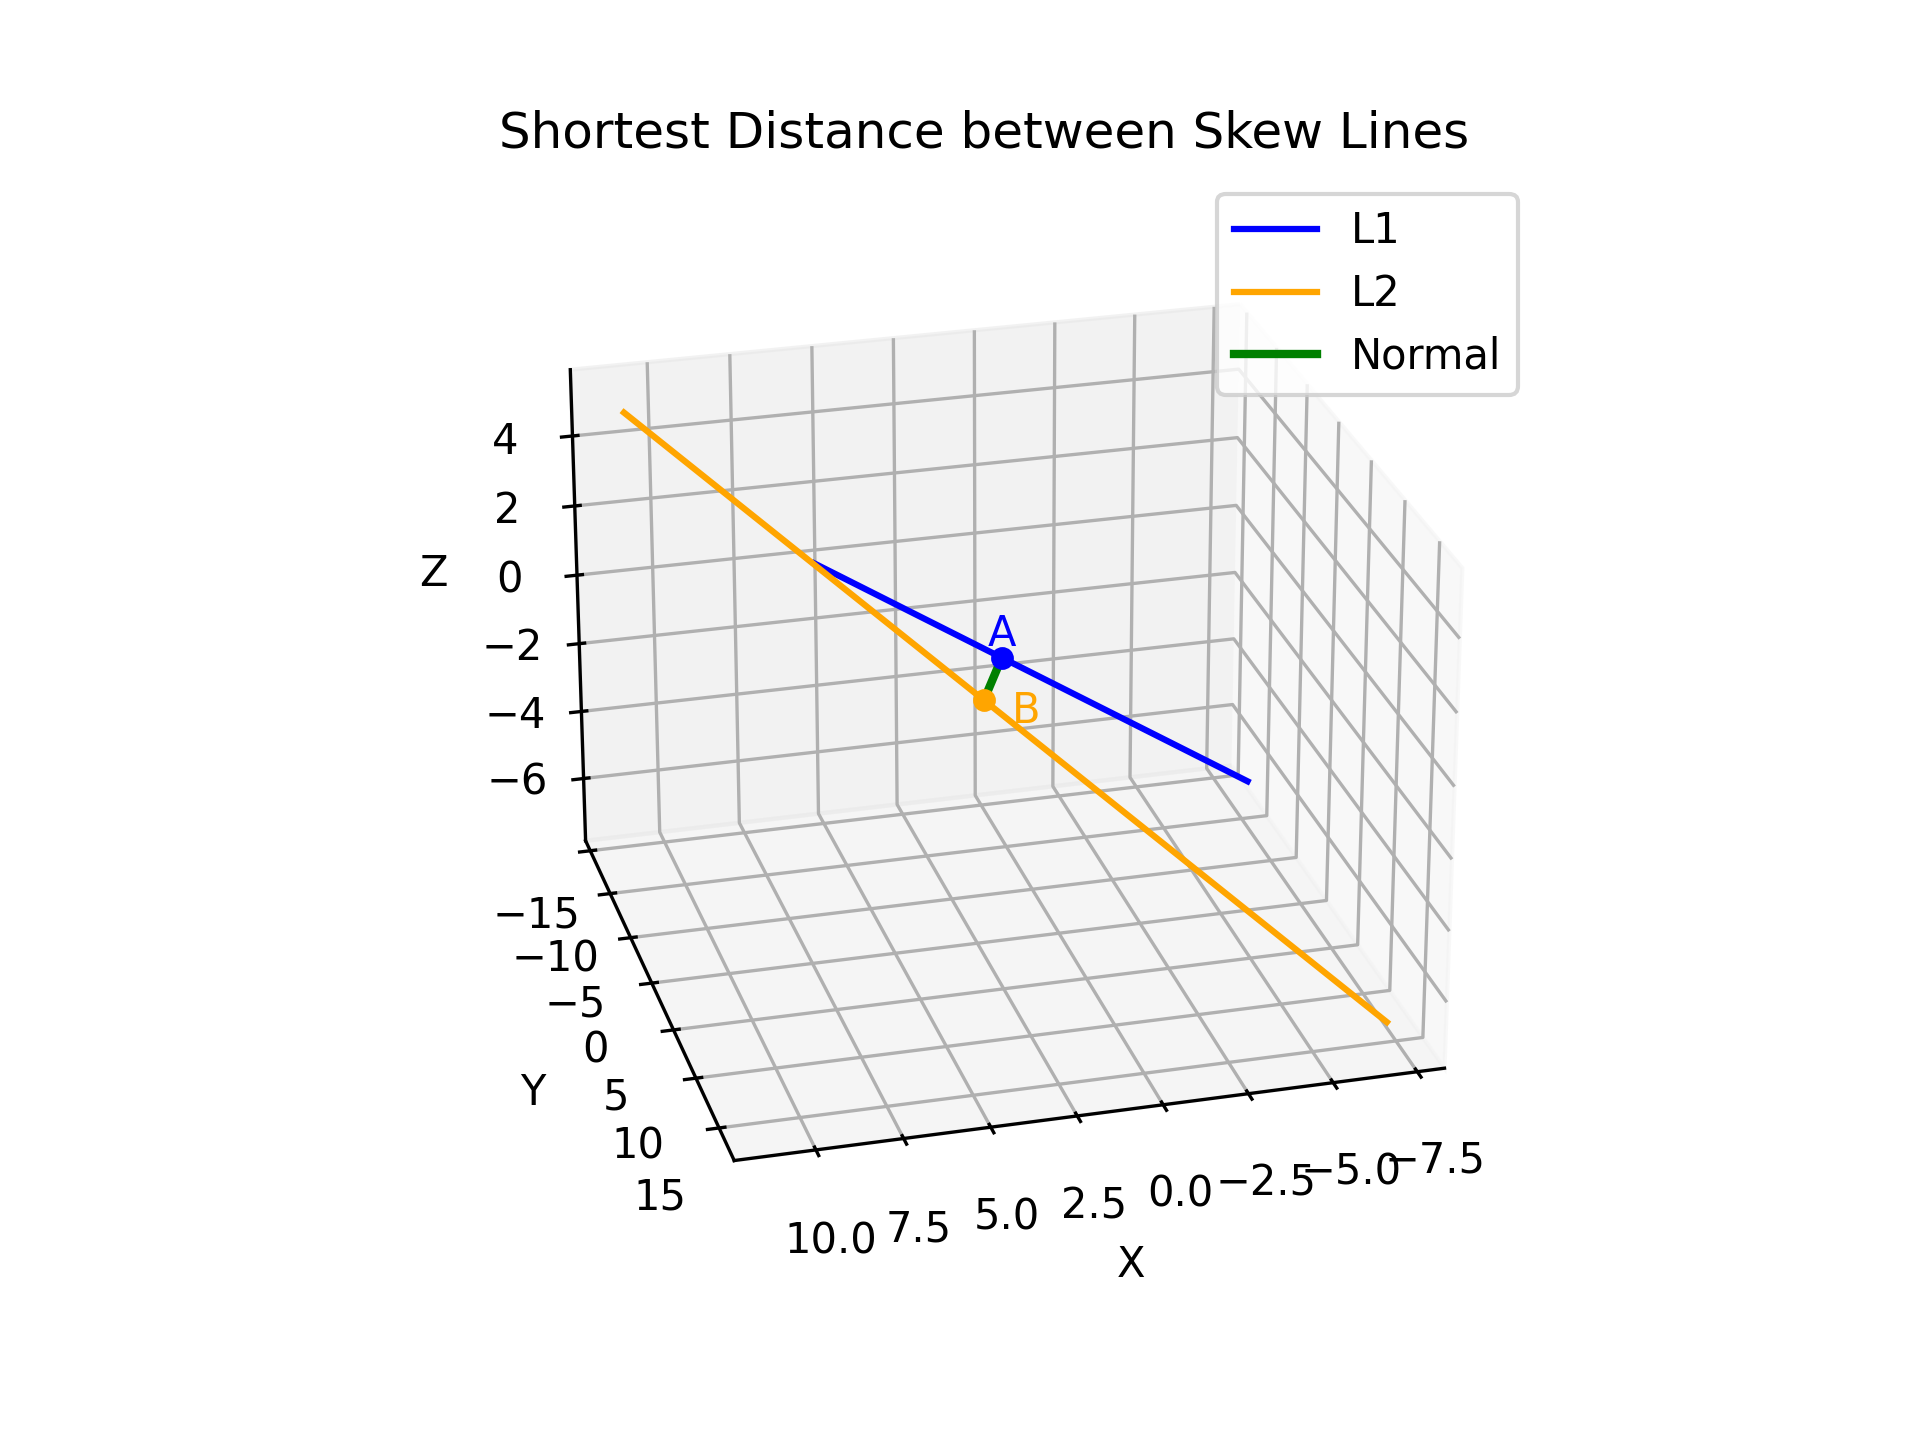
\includegraphics[width=0.7\linewidth]{figs/fig.png}
    \caption{}
    \label{fig:3DVectors}
\end{figure}
\end{frame}

% Python code 1
\begin{frame}[fragile]{Python Code: plot.py (Native)}
\begin{lstlisting}[language=Python]
import numpy as np
import matplotlib.pyplot as plt
from mpl_toolkits.mplot3d import Axes3D

A_start = np.array([1, 1, 0], dtype=np.float64)  # Point A in L1
m1 = np.array([2, -1, 1], dtype=np.float64)      # Direction vector of L1

B_start = np.array([2, 1, -1], dtype=np.float64) # Point B in L2
m2 = np.array([3, -5, 2], dtype=np.float64)      # Direction vector of L2

k1_closest = 25/59
k2_closest = 7/59

point_A = A_start + k1_closest * m1   # Point on L1
point_B = B_start + k2_closest * m2   # Point on L2

shortest_dist = np.linalg.norm(point_B - point_A)
print(f"Shortest distance between the lines = {shortest_dist:.3f}")
\end{lstlisting}
\end{frame}


\begin{frame}[fragile]{Python Code (Native Implementation – plot.py)}
\begin{lstlisting}[language=Python]
kappa_range = np.linspace(-3, 3, 100)
mu_range = np.linspace(-3, 3, 100)

L1_points = np.array([A_start + k * m1 for k in kappa_range])
L2_points = np.array([B_start + k * m2 for k in mu_range])

# --- Plotting ---
fig = plt.figure()
ax = fig.add_subplot(111, projection='3d')

# Plot the two lines
ax.plot(L1_points[:,0], L1_points[:,1], L1_points[:,2], 'b', label='L1')
ax.plot(L2_points[:,0], L2_points[:,1], L2_points[:,2], 'orange', label='L2')

# Plot shortest distance segment
ax.plot([point_A[0], point_B[0]],
        [point_A[1], point_B[1]],
        [point_A[2], point_B[2]], 'g', linewidth=2, label='Normal')
\end{lstlisting}
\end{frame}

\begin{frame}[fragile]{Python Code (Native Implementation – plot.py)}
\begin{lstlisting}[language=Python]
ax.scatter(*point_A, color='b')
ax.scatter(*point_B , color='orange')
ax.text(*point_A + 0.5, "A", fontsize=10, color='b')
ax.text(*point_B - 1.0, "B", fontsize=10, color='orange')

ax.set_xlabel('X')
ax.set_ylabel('Y')
ax.set_zlabel('Z')
ax.view_init(elev=25, azim =75)
ax.legend()
ax.set_title("Shortest Distance between Skew Lines")
plt.savefig("fig.png", dpi=300)
plt.show()
\end{lstlisting}
\end{frame}


\begin{frame}[fragile]{C Code (Shared Library – findlinepoints.c)}
\begin{lstlisting}[language=C]
#include <stdio.h>
#include <math.h>

// Function to compute dot product of 3D vectors
double dot(double a[3], double b[3]) {
    return a[0]*b[0] + a[1]*b[1] + a[2]*b[2];
}

// Function to compute cross product of 3D vectors
void cross(double a[3], double b[3], double result[3]) {
    result[0] = a[1]*b[2] - a[2]*b[1];
    result[1] = a[2]*b[0] - a[0]*b[2];
    result[2] = a[0]*b[1] - a[1]*b[0];
}

// Function to compute norm (magnitude)
double norm(double v[3]) {
    return sqrt(v[0]*v[0] + v[1]*v[1] + v[2]*v[2]);
}


\end{lstlisting}
\end{frame}

\begin{frame}[fragile]{C Code (Shared Library – findlinepoints.c)}
\begin{lstlisting}[language=C]
double find_shortest_distance(double *A_start, double *m1,
                              double *B_start, double *m2,
                              double *pointA, double *pointB)
{
    // Compute dot products
    double m1m1 = dot(m1, m1);
    double m2m2 = dot(m2, m2);
    double m1m2 = dot(m1, m2);

    // Compute RHS vector (A2 - A1)
    double AB[3] = { B_start[0] - A_start[0],
                     B_start[1] - A_start[1],
                     B_start[2] - A_start[2] };

    double rhs1 = dot(AB, m1);
    double rhs2 = dot(AB, m2);
\end{lstlisting}
\end{frame}

\begin{frame}[fragile]{C Code (Shared Library – findlinepoints.c)}
\begin{lstlisting}[language=C]
 // Solve for lambda (k1) and mu (k2)
    double det = (m1m1 * (-m2m2)) - (-m1m2 * m1m2);
    double lam = (rhs1 * (-m2m2) - (-m1m2) * rhs2) / det;
    double mu  = (m1m1 * rhs2 - m1m2 * rhs1) / det;

    // Compute points of closest approach
    for (int i = 0; i < 3; i++) {
        pointA[i] = A_start[i] + lam * m1[i];
        pointB[i] = B_start[i] + mu * m2[i];
    }

    // Compute shortest distance
    double diff[3] = { pointB[0] - pointA[0],
                       pointB[1] - pointA[1],
                       pointB[2] - pointA[2] };

    return norm(diff);
}
\end{lstlisting}
\end{frame}

% Python code 2
\begin{frame}[fragile]{Python Code: call.py (C + Python)}
\begin{lstlisting}[language=Python]
import ctypes
import numpy as np
import matplotlib.pyplot as plt
from mpl_toolkits.mplot3d import Axes3D

lib = ctypes.CDLL("./find_shortest_distance.dll")

lib.find_shortest_distance.argtypes = [
    np.ctypeslib.ndpointer(dtype=np.float64, ndim=1, shape=(3,)),
    np.ctypeslib.ndpointer(dtype=np.float64, ndim=1, shape=(3,)),
    np.ctypeslib.ndpointer(dtype=np.float64, ndim=1, shape=(3,)),
    np.ctypeslib.ndpointer(dtype=np.float64, ndim=1, shape=(3,)),
    np.ctypeslib.ndpointer(dtype=np.float64, ndim=1, shape=(3,)),
    np.ctypeslib.ndpointer(dtype=np.float64, ndim=1, shape=(3,))
]
lib.find_shortest_distance.restype = ctypes.c_double
\end{lstlisting}
\end{frame}

\begin{frame}[fragile]{Python Code (C Integrated – call.py)
}
\begin{lstlisting}[language=Python]
A_start = np.array([1, 1, 0], dtype=np.float64)
m1 = np.array([2, -1, 1], dtype=np.float64)
B_start = np.array([2, 1, -1], dtype=np.float64)
m2 = np.array([3, -5, 2], dtype=np.float64)

pointA = np.zeros(3, dtype=np.float64)
pointB = np.zeros(3, dtype=np.float64)

dist = lib.find_shortest_distance(A_start, m1, B_start, m2, pointA, pointB)
print(f"Shortest distance = {dist:.3f}")
print("Closest point on L1 (A):", pointA)
print("Closest point on L2 (B):", pointB)

kappa_range = np.linspace(-3, 3, 100)
mu_range = np.linspace(-3, 3, 100)

L1_points = np.array([A_start + k * m1 for k in kappa_range])
L2_points = np.array([B_start + k * m2 for k in mu_range])
\end{lstlisting}
\end{frame}

\begin{frame}[fragile]{Python Code (C Integrated – call.py)
}
\begin{lstlisting}[language=Python]
fig = plt.figure()
ax = fig.add_subplot(111, projection='3d')

ax.plot(L1_points[:,0], L1_points[:,1], L1_points[:,2], 'b', label='L1')
ax.plot(L2_points[:,0], L2_points[:,1], L2_points[:,2], 'orange', label='L2')

ax.plot([pointA[0], pointB[0]], [pointA[1], pointB[1]], [pointA[2], pointB[2]],
        'g', linewidth=2, label='Shortest distance')

ax.scatter(*pointA, color='b')
ax.scatter(*pointB, color='orange')
ax.text(*pointA +0.5, "A", fontsize=10, color='b')
ax.text(*pointB - 1.0, "B", fontsize=10, color='orange')

ax.set_xlabel('X')
ax.set_ylabel('Y')
ax.set_zlabel('Z')
ax.legend()
\end{lstlisting}
\end{frame}

\begin{frame}[fragile]{Python Code (C Integrated – call.py)
}
\begin{lstlisting}[language=Python]
ax.set_title("Shortest Distance Between Two Skew Lines ")
plt.savefig("fig_call.png", dpi=300)
plt.show()
\end{lstlisting}
\end{frame}


\end{document}



